We implemented three example user applications using the SimpleChubby service,
namely leader election, double barrier, and group membership.
These applications use the API described in Section~\ref{section:api},
and are able to survive both client and server failures. They demonstrate
that the functionality is correct and the interface is easy to use.

\subsection{Leader Election}

\begin{figure*}
\centering
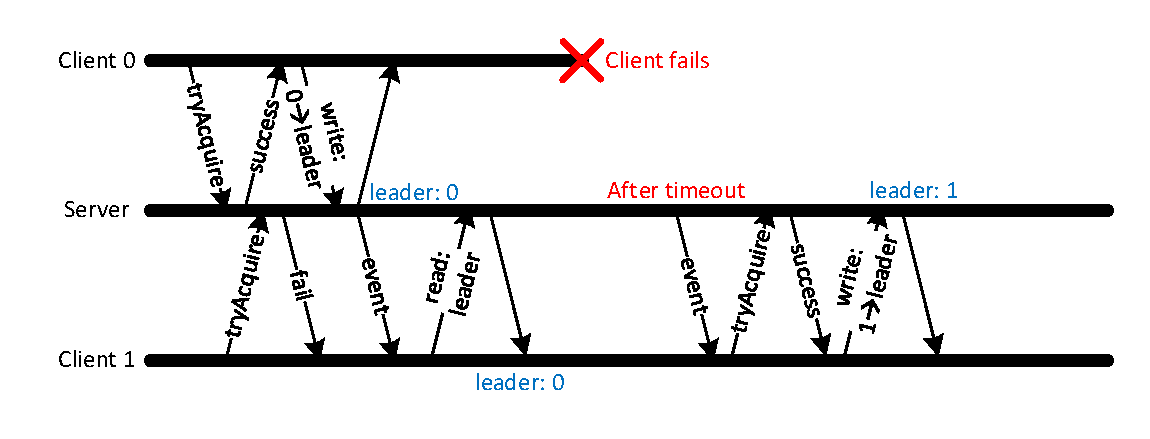
\includegraphics[width=0.8\textwidth]{leader_elect.pdf}
\caption{Leader election. Two clients compete to be the leader. Client 0 wins,
write itself into file ``leader'', but fails later. The server reclaims the
lock and notifies client 1, which becomes the new leader after acquiring the lock.}
\label{fig:leader_elect}
\end{figure*}

Leader election is an application that elects one out of a given group
of clients as the leader. At any given time, at most one client among the
group can be elected as the leader, and other clients should be able to
find out who is the leader, if it exists.

We implement leader election as shown in Figure~\ref{fig:leader_elect}:
all clients open a single
specified file and try to acquire its lock. The one who succeeds becomes
the leader, and write its identity into the file. Others read the file
to figure out who is the leader. The leader continues to hold the lock.
Also, all clients subscribe to the ``lock state changed'' event, in order
to compete for the new leader when the current leader dies. Clients also
subscribe to the ``file content modified'' event to read out the new
leader when changed.

\subsection{Double Barrier}

\begin{figure*}
\centering
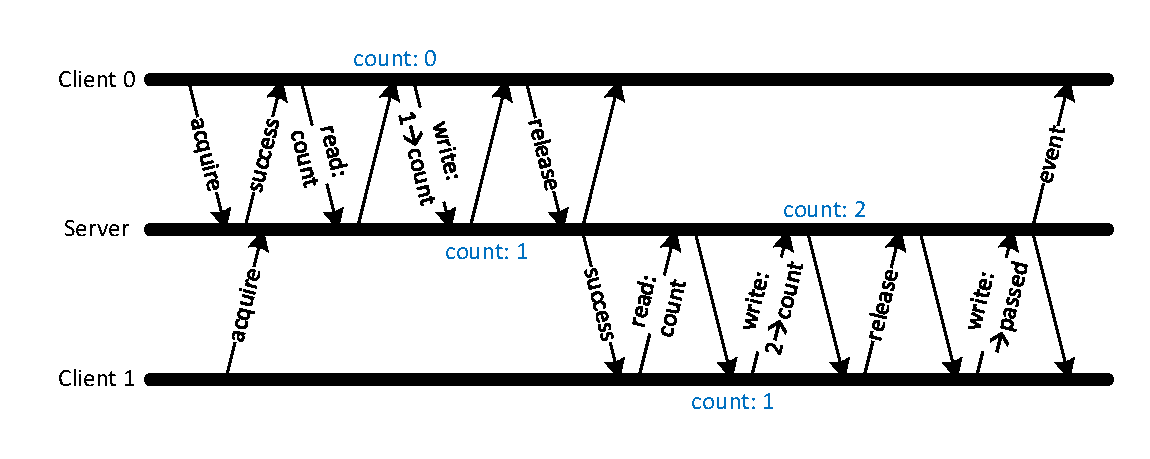
\includegraphics[width=0.8\textwidth]{barrier.pdf}
\caption{Barrier with two clients. Client 0 comes first and set the ``count'' file
content to be 1. Client 1 comes later and set the ``count'' file content to be 2.
Client 2 finds the requirement for the barrier is satisfied and writes to ``pass'' file,
which ends the barrier by delivering events to all clients.}
\label{fig:barrier}
\end{figure*}

Double barriers enable a given number of clients to synchronize at the
beginning and the end of a computation region. When the number of processes
that have joined the barrier reaches the specified number, all processes
start their computation, and leave the barrier together once they have all
finished.

In SimpleChubby, double barrier is implemented using two (single) barriers.
We implement the barrier as shown in Figure~\ref{fig:barrier}: all clients open, lock, and update
one ``count'' file that store with the number of clients reaching the barrier.
Then they wait until a ``file content modified'' event happens with another
``passed'' file. When the last client finds out that the required number
achieves, it writes to the ``passed'' file to trigger the event, and cleans
up the ``count'' file.

\subsection{Group Membership}

Group membership allows all the members inside a specific group to monitor
the group membership changes, such as new member added, normal member leaving,
or member failure.

We implement this application using the directory feature in SimpleChubby.
When entering the group, the member creates a ephemeral file in the group
directory with the name of itself, and query the directory content to get
the list of all members. The members also subscribe to the ``directory content
modified'' event of the group directory, so that they can obtain the most
up-to-date membership. When leaving the group, the member deletes its file.
The ephemeral feather ensures the correctness even at failure.



